\documentclass[en,license=none]{../../../eplsummary}
\usepackage{listings}
\usepackage{../../../eplcommon}

\usetikzlibrary{calc, trees, positioning, arrows, shapes, shapes.multipart, shadows, matrix, decorations.pathreplacing, decorations.pathmorphing}
\usetikzlibrary{arrows,shapes,snakes,automata,backgrounds,petri}

\hypertitle{Cloud Computing}{7}{INGI}{2145}
{Houtain Nicolas, Thibault Gérondal, Kabasele Ndonda Nicolas, Feuillen Gauthier}
{Canini Marco}

\section{Cloud computing}
\input{parts/01-cloud}

\section{Design for scale}
A system is scalable if it can easily adapt to 
increased (or reduced) demand. Scalablity
is usually limited by some sort of bottleneck.

\subsection{Parallelism programming}

\subsubsection{Vocabulary}
\begin{description}
    \item[Parallelism]: refers to techniques to make programs faster by
        performing several computations in parallel.

    \item[Concurrency]: is the composition of independently executing
        computations.

\end{description}

\subsubsection{Parallelization}
\begin{itemize}
    \item \textbf{Amdahl's law}:

        \begin{tabular}{m{0.5\linewidth}m{0.5\linewidth}}
            $$\quad S = \frac{1}{\alpha +
            \frac{1-\alpha}{N}}$$ where $\alpha$ is the sequential part and $N$ the
            number of cores.
            &
            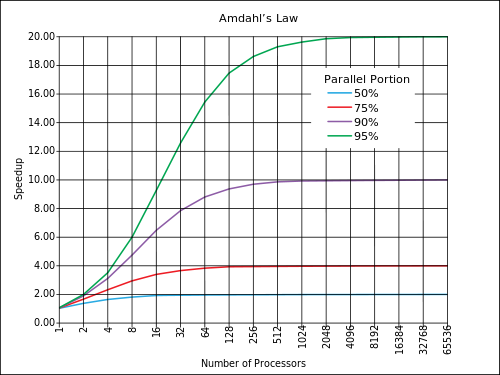
\includegraphics[width=6cm]{img/amdahl.png}
        \end{tabular}

        The coarse-grain (low rate communication) opposed to fine-grain (high rate) 
        parallelism is more efficient because it limits the communication and 
        coordination overheads by allow bigger task.

    \item \textbf{Dependencies}: Some task need to be after other which limits the degree of 
        parallelism. $\rightarrow$ Scheduling problem
\end{itemize}

\subsubsection{Synchronization}
Synchronization is needed when state is updated by different entities
(threads,process,servers,...)
\begin{description}
    \item[Race condition]: Result of the computation depends on the exact
        timing of the two threads of execution,i.e, the order in which instruction 
        are executed.

\end{description}

\subsubsection{Architecture}
\begin{itemize}
    \item Symmetric multiprocessing (SMP): all processors share same memory.

        \begin{tabular}{m{0.6\linewidth}m{0.3\linewidth}}
            \begin{itemize} 
                \item[+] Simplicity and easy to load balance 
                \item[-] Scalability limited and expensive
            \end{itemize}
            &
            \begin{tiny}
                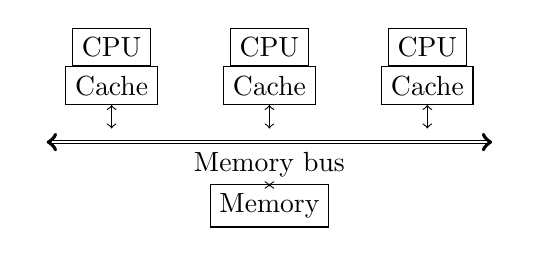
\begin{tikzpicture}
                    \node[draw, rectangle] (1) {CPU};
                    \node[draw, rectangle] (2) [right=of 1] {CPU};
                    \node[draw, rectangle] (3) [right=of 2] {CPU};

                    \node[draw, rectangle] (11) [below=0cm of 1] {Cache};
                    \node[draw, rectangle] (21) [below=0cm of 2] {Cache};
                    \node[draw, rectangle] (31) [below=0cm of 3] {Cache};

                    \node (12) [below=0.3cm of 11] {};
                    \node (22) [below=0.3cm of 21] {};
                    \node (32) [below=0.3cm of 31] {};

                    \node (tmp) [below left= -0.2cm and 0.7cm of 12] {};
                    \node (tmp2) [below right=-0.2cm and 0.7cm of 32] {};

                    \draw (tmp) edge[double, <->] node[below](p) {Memory bus} (tmp2);
                    \draw (12) edge[<->] (11);
                    \draw (22) edge[<->] (21);
                    \draw (32) edge[<->] (31);

                    \node[draw, rectangle] (mem) [below=1.0cm of 21] {Memory};
                    \draw (mem) edge[<->] (p);
                \end{tikzpicture}
            \end{tiny}
        \end{tabular}

    \item Non Uniform memory architecture (NUMA)

        \begin{tabular}{m{0.6\linewidth}m{0.3\linewidth}}
            \begin{itemize} 
                \item[+] Better scalability and faster memory
                \item[-] Complicates programming and scalability limited
            \end{itemize}
            &
            \begin{tiny}
                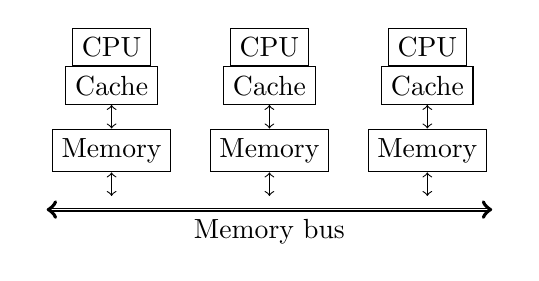
\begin{tikzpicture}
                    \node[draw, rectangle] (1) {CPU};
                    \node[draw, rectangle] (2) [right=of 1] {CPU};
                    \node[draw, rectangle] (3) [right=of 2] {CPU};

                    \node[draw, rectangle] (11) [below=0cm of 1] {Cache};
                    \node[draw, rectangle] (21) [below=0cm of 2] {Cache};
                    \node[draw, rectangle] (31) [below=0cm of 3] {Cache};

                    \node[draw, rectangle] (12) [below=0.3cm of 11] {Memory};
                    \node[draw, rectangle] (22) [below=0.3cm of 21] {Memory};
                    \node[draw, rectangle] (32) [below=0.3cm of 31] {Memory};

                    \node (13) [below=0.3cm of 12] {};
                    \node (23) [below=0.3cm of 22] {};
                    \node (33) [below=0.3cm of 32] {};

                    \node (tmp) [below left= -0.2cm and 0.7cm of 13] {};
                    \node (tmp2) [below right=-0.2cm and 0.7cm of 33] {};

                    \draw (tmp) edge[double, <->] node[below](p) {Memory bus} (tmp2);
                    \draw (12) edge[<->] (11);
                    \draw (22) edge[<->] (21);
                    \draw (32) edge[<->] (31);

                    \draw (12) edge[<->] (13);
                    \draw (22) edge[<->] (23);
                    \draw (32) edge[<->] (33);
                \end{tikzpicture}
            \end{tiny}
        \end{tabular}

    \item Shared Nothing

        \begin{tabular}{m{0.6\linewidth}m{0.3\linewidth}}
            \begin{itemize} 
                \item[+] Nice scalability
                \item[-] Requires different programming model
            \end{itemize}
            &

            \begin{tiny}
                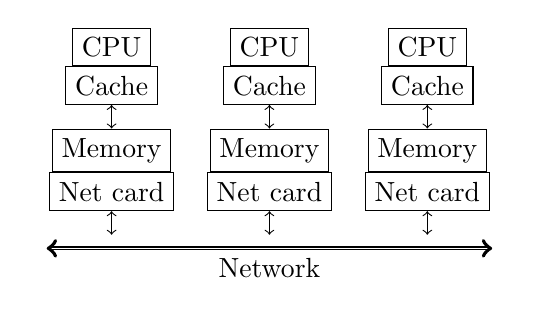
\begin{tikzpicture}
                    \node[draw, rectangle] (1) {CPU};
                    \node[draw, rectangle] (2) [right=of 1] {CPU};
                    \node[draw, rectangle] (3) [right=of 2] {CPU};

                    \node[draw, rectangle] (11) [below=0cm of 1] {Cache};
                    \node[draw, rectangle] (21) [below=0cm of 2] {Cache};
                    \node[draw, rectangle] (31) [below=0cm of 3] {Cache};

                    \node[draw, rectangle] (12) [below=0.3cm of 11] {Memory};
                    \node[draw, rectangle] (22) [below=0.3cm of 21] {Memory};
                    \node[draw, rectangle] (32) [below=0.3cm of 31] {Memory};

                    \node[draw, rectangle] (14) [below=0cm of 12] {Net card};
                    \node[draw, rectangle] (24) [below=0cm of 22] {Net card};
                    \node[draw, rectangle] (34) [below=0cm of 32] {Net card};

                    \node (13) [below=0.3cm of 14] {};
                    \node (23) [below=0.3cm of 24] {};
                    \node (33) [below=0.3cm of 34] {};

                    \node (tmp) [below left= -0.2cm and 0.7cm of 13] {};
                    \node (tmp2) [below right=-0.2cm and 0.7cm of 33] {};

                    \draw (tmp) edge[double, <->] node[below](p) {Network} (tmp2);
                    \draw (12) edge[<->] (11);
                    \draw (22) edge[<->] (21);
                    \draw (32) edge[<->] (31);

                    \draw (13) edge[<->] (14);
                    \draw (23) edge[<->] (24);
                    \draw (33) edge[<->] (34);
                \end{tikzpicture}
            \end{tiny}
        \end{tabular}

\end{itemize}


\subsection{Distributed programming}

\subsubsection{Vocabulary}
\begin{description}
    \item[Faults]: Some component is not working correctly
    \item[Failure]: System as a whole is not working correctly
\end{description}

\subsubsection{Wide-area network}
The transfert speed for some data are defined by some attributs:
\begin{enumerate}
    \item Propagation delay
    \item Bottlenecks capacity on the path
    \item Queueing delay, loss, reordering, congestion, rtt 
        (take in account by TCP)
\end{enumerate}

$\rightarrow$ wide-area networks complicates the communication and faults are
more common

\subsubsection{Faults}

Fault are a common event in distributed system and some faults
are correlated.

\begin{itemize}
    \item \textbf{Crash faults}: node simply stop
    \item \textbf{Rational behavior}: owner manipulates node to increase profit
        (ex: lies on the routes to have traffic through it's own AS)
    \item \textbf{Byzantine faults}: faulty node could do anything (ex: stop, send spam,
        attack other, tell lies,...)
\end{itemize}

To prevent fault, we can \textit{prevent} them by using verification,
\textit{detect} them or \textit{mask} them by using replicas. The problem of
using \textbf{replicas} is to be able to maintain consistency between them!

\subsubsection{Consistency}

\begin{itemize}
    \item \textbf{Strong consistency}: After update completes, all subsequent
        accesses will return the updated value

    \item \textbf{Weak consistency}: After update completes, accesses do not
        necessarily return the updated value;; some condition must be satisfied
        first (such as update needs to reach all the replicas)

    \item \textbf{Eventual consistency}: Specific form of weak consistency: If no
        more updates are made to an object, then eventually all reads will return
        the latest value

    \item \textbf{Causal consistency}: If client A has communicated to client B that it
        has updated a data item, a subsequent access by B will return the updated
        value, and a write is guaranteed to supersede the earlier write. Client C
        that has no causal relationship to client A is subject to the normal
        eventual consistency rules

    \item \textbf{Read-your-writes consistency}: Client A, after it has updated a data
        item, always accesses the updated value and will never see an older
        value.

    \item \textbf{Session consistency}: Like previous case but in the context of a
        session, for as long as the sessions remains alive.

    \item \textbf{Monotonic read consistency}: If client A has has seen a particular value
        for the object, any subsequent accesses will never return any previous
        values

    \item \textbf{Monotonic write consistency}: In this case the system guarantees to
        serialize the writes by the same process
\end{itemize}

We can combine them, and monotonic reads + read-your-write are most desirable
than eventual consistency.

\paragraph{Storage system consistency: example}

We have N nodes that can store data.
To write a value: Pick W replicas and write the value to each, using a fresh timestamp
To read a value:
\begin{itemize}
    \item Pick R replicas and read the value from each
    \item Return the value with the highest timestamp
    \item If any replicas had a lower timestamp, send them the newer value
\end{itemize}

\begin{tabular}{m{4cm}m{10cm}}
    Strong consistency :&
\begin{description}
    \item[Majority quorum] Always write to and read from a majority of nodes. At least one node knows the most recent value. tolerate up to $\ceil{N/2} - 1$ crashes. But have to read/write $\floor{N/2} + 1$ values.
    \item[Read/write quorums] Read R nodes, write W nodes, s.t. R + W > N. Adjust performance of reads/writes. But availability can suffer.

        \begin{tabular}{m{3cm}m{12cm}}
            \includegraphics[width=3cm]{img/replicas} &
            \includegraphics[width=7cm]{img/replicas2}
            \begin{itemize}
                \item[$\rightarrow$] Strong consistency
            \end{itemize} \\
        \end{tabular}
    \item[Consensus solutions] Paxos (for crash faults), PBFT (for Byzantine faults). Idea : Correct replicas ``outvote'' faulty ones.
\end{description}
\end{tabular}


The cap theorem : We can get at most two out of the three
\begin{itemize}
    \item Consistency : All clients single up-to-data copy of the data, even in the presence of concurrent updates
    \item Availability: Every request (including updates) received by a non-failing node in the system must result in a response, even when faults occur
    \item Partition-tolerance: Consistency and availability hold even when the network partitions
\end{itemize}

Dealing with network partitions when a partition is cut : Enter an explicit partition mode that can limit some operations.


\includegraphics[width=\linewidth]{img/part}




\paragraph{Consensus}
\begin{enumerate}
    \item Clients send requests to each of the replicas
    \item Replicas coordinate and each return a result
    \item Client chooses one of the results, e.g., the one that is 
        returned by the largest number of replicas
    \item If a small fraction of the replicas returns the wrong result, or 
        no result at all, they are 'outvoted' by the other replicas
\end{enumerate}


\subsubsection{CAP theorem}
\begin{center}
    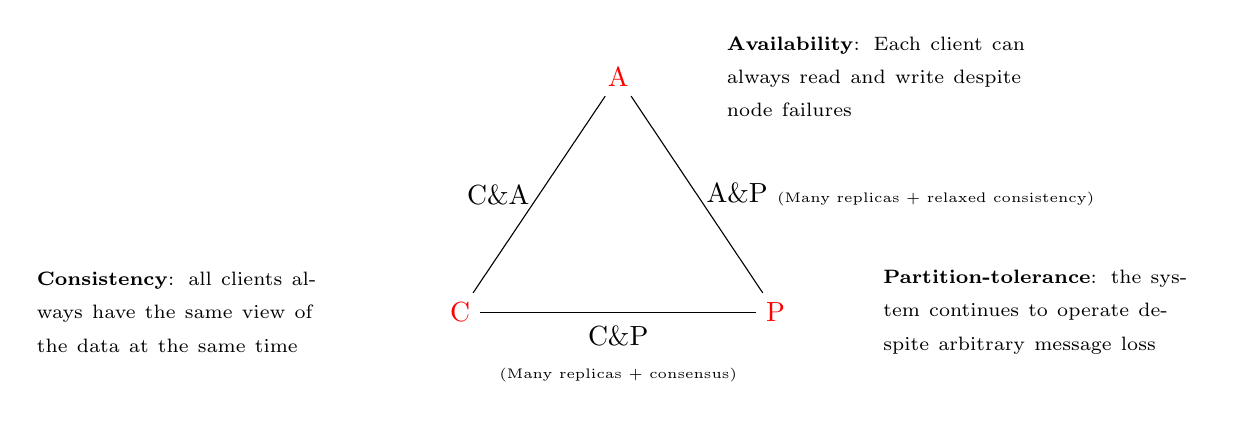
\begin{tikzpicture}
        \node (A) {\textcolor{red}{A}};
        \node (C) [below left= 2.5cm and 1.5cm of A] {\textcolor{red}{C}};
        \node (P) [below right= 2.5cm and 1.5cm of A] {\textcolor{red}{P}};

        \node[right =1cm of A, text width=4cm] {\scriptsize \textbf{Availability}: Each client can always read
        and write despite node failures};

        \node[left =1cm of C, text width=4cm] {\scriptsize \textbf{Consistency}: all clients always have the
        same view of the data at the same time};

        \node[right =1cm of P, text width=4cm] {\scriptsize \textbf{Partition-tolerance}: the
        system continues to operate despite arbitrary message loss};

        \draw (A) edge[-] node[left] {C\&A} (C);
        \draw (A) edge[-] node[right] {A\&P \tiny (Many replicas + relaxed consistency)} (P);
    \draw (C) edge[-] node[below] {\begin{tabular}{c}C\&P\\ \tiny (Many replicas + consensus) \end{tabular}} (P);
    \end{tikzpicture}
\end{center}


\paragraph{Actually}, we have a lot of partition and we have a trade-off
between C and A. \textbf{ACID} (atomicity, consistency, isolation, durability)
become \textbf{BASE} (basically available, soft-state, eventually consistent).


\subsection{Structure}
\begin{figure}[!h]
    \centering
    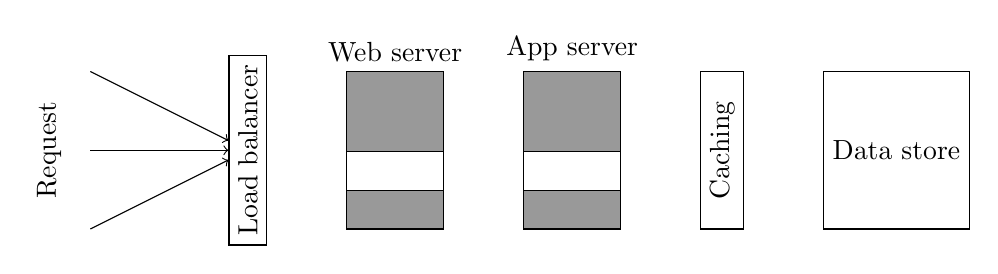
\begin{tikzpicture}

        \node[draw, rectangle, minimum height= 2cm] (L) {\rotatebox{90}{Load balancer}};
        \node[draw, rectangle, fill=black!40, minimum height= 2cm, text width=1cm, right= of L] (W) {};
        \node[draw, rectangle, fill= white, minimum height= 0.5cm, text width=1cm, below=-1cm of W] (W1) {};
        \node[above=0cm of W] (1) {Web server};

        \node[draw, rectangle, fill=black!40, minimum height= 2cm, text width=1cm, right= of W] (A) {};
        \node[draw, rectangle, fill=white, minimum height= 0.5cm, text width=1cm, below=-1cm of A] (A1) {};
        \node[above=0cm of A] (1) {App server};

        \node[draw, rectangle, minimum height= 2cm, right= of A] (C) {\rotatebox{90}{Caching}};
        \node[draw, rectangle, minimum height= 2cm, right= of C] (D) {Data store};

        \draw[->] (-2, 0) -- (L);
        \draw[->] (-2, -1) -- (L);
        \draw[->] (-2, 1) -- (L);

        \node[left=2cm of L] (R) {\rotatebox{90}{Request}};

    \end{tikzpicture}
    \caption{Cloud structure with 
        caching which is central to responsiveness. Cached data are used by the inner
    services to shield them form online load}
\end{figure}

\begin{itemize}
    \item \textbf{Stateless server}: Views a client request as an independent 
        transaction and responds to it


        Easy to scale and more robust because instance failure does not require
        overheas restoring state

    \item \textbf{Statefull server}: Scaling is challenging because we need to maintains 
        the state.

        \paragraph{Traditionnal approach is replication}:

        \begin{tabular}{m{12cm}m{5cm}}
            \begin{itemize}
                \item Data is written to a \textit{master server} and then
                    replicated to one or more \textit{slave servers}
                    (synchronously or asynchronously)
                \item Read operations can be handled by the slaves
            \end{itemize}
            But in this case, master becomes the write bottleneck and single point of failure.
            &
            \centering
            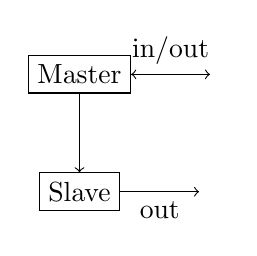
\begin{tikzpicture}
                \node[draw, rectangle] (M) {Master};
                \node[draw, rectangle, below=1cm of M] (S) {Slave};
                \node (I) [right= of M] {};
                \node (O) [right= of S] {};

                \draw[->, double] (I) edge node[above] {in/out} (M);
                \draw[<-, double] (I) edge (M);
                \draw[<-, double] (O) edge node[below] {out}(S);
                \draw[->, double] (M) edge (S);
            \end{tikzpicture}
        \end{tabular}


        \paragraph{Sharding with partitionning}
        The idea is to split data between multiple 
        machines and have a way to make sure that
        the data is available on the right place.
        Typically, define a \textbf{sharding key} and create a \textbf{shard mapping}.

        \begin{tabular}{cm{10cm}}
            This allow to have &
            \begin{itemize}
                \item a really high availability
                \item increase read and write throughput
                \item the possibility 
                    of doing more work in parallel within the application server.
                \item[But] the challenge is to find a good partitionning scheme.
            \end{itemize}
        \end{tabular}

        \textbf{Sharding} is not only for partitioning data 
        within a database, but can also be use to partition data across caching 
        servers (memcached, redis).
\end{itemize}

\paragraph{First-tier parallelism}
Parallelism is vital for fast interactive services, and 
parallel actions must focus on the \textbf{critical path}. This is the
contributor delay for the response delay and do
not care about asynchronous that are shortly.

\begin{center}
    \includegraphics[width=9cm]{img/critical}
\end{center}


Note that update for replicas are typically done in asynchronous way, so we
might not experience much delay on the critical path.

$\rightarrow$ Asynchronous operations decouple systems and 
enable quicker responses at the expense strong 
consistency.
Indeed, this can rise some issues which result in inconsistency:
\begin{itemize}
    \item We don't know in which order replicas applying the update
    \item The leader can crash before replicas change and lose some
        update
\end{itemize}





\section{Cloud storage}
\input{parts/03-storage}

\section{MapReduce}

\begin{figure}[!h]
    \centering
    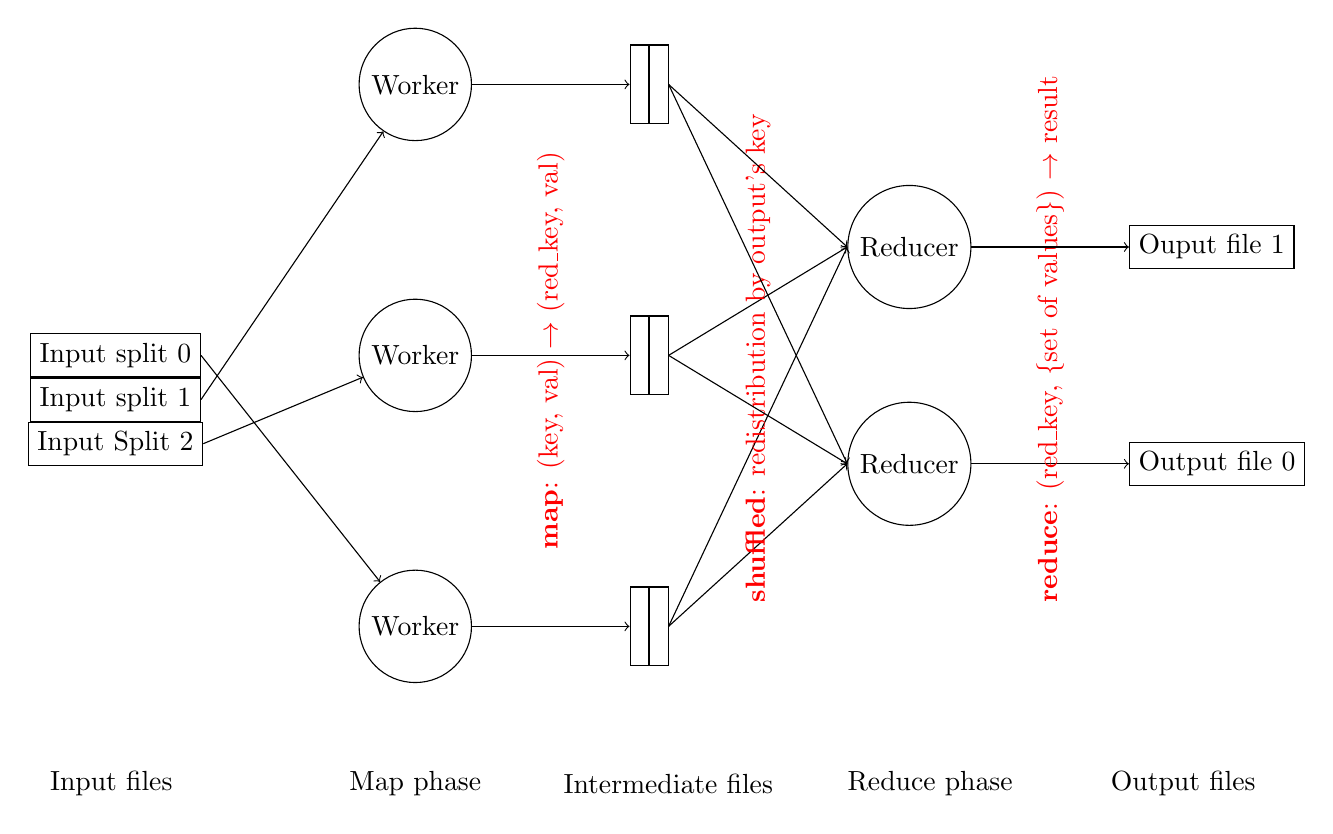
\begin{tikzpicture}[node distance=2cm]
        \node[draw, rectangle] (I0) {Input split 0};
        \node[draw, rectangle, below=0cm of I0] (I1) {Input split 1};
        \node[draw, rectangle, below=0cm of I1] (I2) {Input Split 2};

        \node[draw, circle, right=of I0 ] (W2) {Worker};
        \node[draw, circle, below=of W2 ] (W1) {Worker};
        \node[draw, circle, above=of W2 ] (W3) {Worker};

        \node[draw, minimum height=1cm,rectangle, right=of W1 ] (F1) {};
        \node[draw, minimum height=1cm, rectangle, right=of W2 ] (F2) {};
        \node[draw, minimum height=1cm, rectangle, right=of W3 ] (F3) {};

        \node[draw, rectangle, minimum height=1cm, right=0cm of F1 ] (FF1) {};
        \node[draw, rectangle, minimum height=1cm,right=0cm of F2 ] (FF2) {};
        \node[draw, rectangle, minimum height=1cm, right=0cm of F3 ] (FF3) {};

        \node[draw, circle, above right=1cm and 2.5cm of FF1 ] (R1) {Reducer};
        \node[draw, circle, below right=1cm and 2.5cm of FF3 ] (R2) {Reducer};

        \node[draw, rectangle, right=of R1 ] (O1) {Output file 0};
        \node[draw, rectangle, right=of R2 ] (O2) {Ouput file 1};

        \draw (I0.0) edge[->](W1);
        \draw (I1.0) edge[ ->](W3);
        \draw (I2.0) edge[ ->](W2);

        \draw (W1.0) edge[->] (F1.180);
        \draw (W2.0) edge[->] node 
        {\rotatebox{90}{ \textcolor{red}{\textbf{map}: (key, val) $\rightarrow$ (red\_key, val)}}} (F2.180);
        \draw (W3.0) edge[->] (F3.180);

        \draw (FF1.0) edge[->] (R1.180);
        \draw (FF1.0) edge[->] (R2.180);
        \draw (FF2.0) edge[->] node[below=-2.5cm]
        {\rotatebox{90}{ \textcolor{red}{\textbf{shuffled}: redistribution by output's key}}} (R2.180);
        \draw (FF2.0) edge[->] (R1.180);
        \draw (FF3.0) edge[->] (R1.180);
        \draw (FF3.0) edge[->] (R2.180);

        \draw (R1.0) edge[->] node[above=-2cm]
        {\rotatebox{90}{ \textcolor{red}{\textbf{reduce}: (red\_key, \{set of values\}) $\rightarrow$ result}}} (O1.180); 
        \draw (R2.0) edge[->] (O2.180);

        \node[below=1cm of W1] (2) {Map phase};
        \node[left=of 2] (1) {Input files};
        \node[right=0.8cm of 2] (3){Intermediate files};
        \node[right=0.7cm of 3] (4){Reduce phase};
        \node[right=1cm of 4] (5){Output files};


    \end{tikzpicture}

    \centering
    \begin{itemize}
        \item \textbf{File system} distributed across all nodes with replication
        \item \textbf{Driver program} on the master to keeping all node busy
        \item \textbf{Runtime system} which control nodes
    \end{itemize}
    \caption{MapReduce where mapper and reducer should be \textbf{stateless}
    }
\end{figure}


A variety of different tasks can be expressed 
as a single-­pass MapReduce program which are specifically designed
for \textbf{batch operation} over large amounts of data:
\begin{itemize}
    \item filter, collect, aggregate, join on shared element
\end{itemize}

\paragraph{Not for MapReduce}
\begin{itemize}
    \item sorting don't work in the abstract model (but the
        implementation support it)
    \item algorithms that depend on shared global state during 
        processing are difficult to implement.
    \item Process live data at high throughput and low latency

\end{itemize}


\subsection{Failure}
On worker crash we rely on the file system being shared 
across all the nodes. 
\begin{itemize}
    \item If the node wrote its output and then crashed, 
        the file system is likely to have a copy of the complete output.
    \item If the node crashed before finishing its output, the master 
        see that the job isn’t making progress, and restarts the 
        job elsewhere on the system
\end{itemize}

$\Rightarrow$ Hadoop jobs can always complete as long as there is a
worker alive because the master redistribute the jobs to other worker.
(of course, we have fewer nodes to do work...)

Note that the master can't fail to redistribute the jobs.

\subsection{Optimization}

\begin{enumerate}
    \item \textit{locality}: Master tries to do work on nodes that 
        have replicas of the data
    \item \textit{Stragglers}: re-execute slow machines task somewhere else.

    \item \textit{Combiner}: use between mapper and reducer in order to be more efficient.
        Typically, it's job is to pass $(xyz, k)$ instead of $k$ copies of $(xyz, 1)$.
\end{enumerate}

\subsection{Single-Pass algorithm}

\begin{itemize}
	%% Should not the Intersection check the size of the values?
	\item \textbf{Aggreation} Compute 
	\item \textbf{Filtering} Remove item that does not sastifies a property
	\item \textbf{Intersection} Return the intersection bewteen two set (
	remove duplicated value that appears in the two set).
	\item \textbf{Join} Combine two set according to a common properties
\end{itemize}

\subsection{Shuffle}

\begin{itemize}
    \item \textbf{Sorting on key}
        Runtime guarantees that reduce keys will be 
        presented to reduce in sorted order. Shuffle really
        consists of two parts: (1) Partition and (2) Sort.

    \item \textbf{Sorting on value} To sort by value, a composite key containing 
    the value to sort must be used. In that case, the key comparator must take
    into account that the key is composed. 
\end{itemize}

\subsection{Iterative}
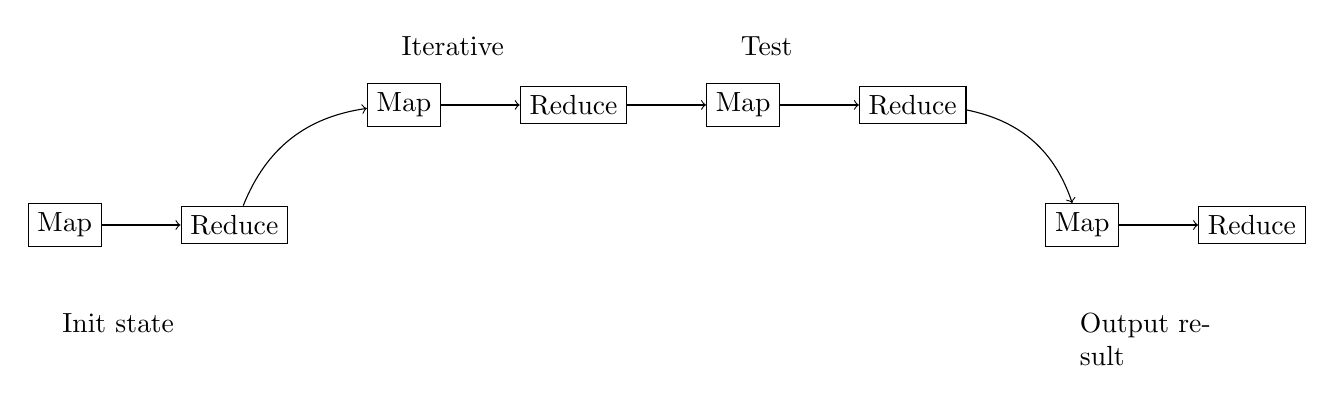
\begin{tikzpicture}
    \node[rectangle, draw] (IM) {Map};
    \node[rectangle, draw, right= of IM] (IR) {Reduce};

    \node[rectangle, draw, above right= of IR] (CM) {Map};
    \node[rectangle, draw, right= of CM] (MR) {Reduce};

    \node[rectangle, draw, right= of MR] (TM) {Map};
    \node[rectangle, draw, right= of TM] (TR) {Reduce};

    \node[rectangle, draw, below right= of TR] (OM) {Map};
    \node[rectangle, draw, right= of OM] (OR) {Reduce};

    \draw (IM) edge[->] node[below=1cm, text width=2cm] {Init state} (IR);
    \draw (CM) edge[->] node[above=0.5cm, text width=2cm] {Iterative} (MR);
    \draw (TM) edge[->] node[above=0.5cm, text width=2cm] {Test} (TR);
    \draw (OM) edge[->] node[below=1cm, text width=2cm] {Output result} (OR);

    \draw (IR) edge[->, bend left] (CM);
    \draw (MR) edge[->, ] (TM);
    \draw (TR) edge[->, bend left] (OM);
\end{tikzpicture}

Iterative MapReduce can be done if the reduce
output is compatible with map input but this require to passing the
entire state and doing a lot of network and disk I/O.


\subsection{Graphs algorithm}
$G = (V, E)$ where $V$ is vertices, $E$ edges of the form $(v_1, v_2, cost, attr)$
where $v_1, v_2 \in V$.

\begin{itemize}
    \item \textbf{Single Source Shortst Path (SSSP)}: based on dijkstra algorithm idea but parallelized.
        \begin{description}
            \item[Init]: for each node $id$, $<\infty, -, \{<succId, cost>\}>$
            \item[Map]: for each node $id$, $<dst, next, \{<succId, cost>\}>$:
                \begin{itemize}
                    \item emit $id$, $<dst, next, \{<succId, cost>\}>$
                    \item for each successor:
                        \begin{itemize}
                            \item emit $succId, <dst+cost, id>$ 
                        \end{itemize}
                \end{itemize}
            \item[Reduce]: emit $id$, $<minDst, nextWithMinDst, \{<succId, cost>\}>$
        \end{description}

        This algorithm is based on a \textit{wave} which go on at each iteration.

    \item \textbf{k-clustering}: the idea is to assign $k$ random centroid and move them 
        until be stable.
        \begin{description}
            \item[Init]: choose random point
            \item[Map]: Assign each point to the closest centroid
                $$S_i^{(t)} = \{ x_j : x_j - m_i^{(t)} \leqslant x_j - m_i^{(* t )} , i* = 1,..., k \}$$
            \item[Reduce]: Recenter with $m_i$ the new centroid for its points
                $$m_i^{(t+1)} = \frac{1}{|S_i^{(t)}|} \sum_{x_j \in S_i^{(t)}} x_j$$
        \end{description}

    \item \textbf{Classification with naïve Bayes}: where it's \textit{naïve} because probability
        of events are independent.
        $$\textrm{Probability messages "XYZ" is SPAM?} = \frac{p(spam) p(containsXYZ | spam)}
        {p(containsXYZ)}$$ 

        \begin{itemize}
            \item \texttt{p(spam)} : Nbr spam email / Nbr email
            \item \texttt{p(containsXYZ)} : Nbr emails with XYZ / Nbr emails
            \item \texttt{p(containsXYZ|spam)} : Nbr emails with XYZ / Nbr emails with XYZ
        \end{itemize}

        \begin{tabular}{m{2cm}cm{13cm}}
            Nbr spam with XYZ &:
            & 
            \begin{description}
                \item[map]: for each message $m <class, \{words\}>$, emit $<word, class> \rightarrow 1$
                \item[reduce]: emit $<word, class> \rightarrow count$
            \end{description}
        \end{tabular}

        \begin{tabular}{m{2cm}cm{12cm}}
            Nbr email with XYZ&:
            & 
            \begin{description}
                \item[map]: for each message $m <class, \{words\}>$, emit $<word> \rightarrow 1$
                \item[reduce]: emit $<word> \rightarrow count$
            \end{description}
        \end{tabular}

    \item \textbf{PageRank}: The idea is to allow $\frac{1}{N}$ vote par page
        at the initialization, and each page vote for all the page it has a
        link to. To ensure fairness, pages voting for more than one page must
        split their vote equally between them. Voting proceeds in rounds: in
        each round, each page has the number of votes it received in the
        previous round.


        \begin{itemize}
            \item \textsc{Random surfer model}: Imagine a random surfer, who starts on a 
                random page and, in each step
                \begin{enumerate}
                    \item Click on a random link on the page with probability $d$ 
                    \item Jump to a random page with probability $1-d$ 
                \end{enumerate}
                The PageRank of a page can be interpreted 
                as the fraction of steps the surfer spends on 
                the corresponding page


            \item \textsc{Naïve PageRank}
                $$rank_i = \sum_{j \in B_i} \frac{1}{N_j} rank_j \quad \textrm{where }N_i \textrm{ is
                the outgoing link of i and} B_i \textrm{ the ingoing link of i}$$ 

                This can't be able to manage vertex which have no outgoing edge.

                \begin{tabular}{m{7cm}m{7cm}}
                    \textbf{Sinks} & \textbf{Hogs}\\
                    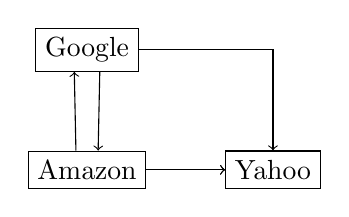
\begin{tikzpicture}
                        \node[rectangle, draw] (G) {Google};
                        \node[rectangle, draw, below= of G] (A) {Amazon};
                        \node[rectangle, draw, right= of A] (Y) {Yahoo};

                        \draw[->] (G) -| (Y);
                        \draw[->] (G.300) -- (A.60);
                        \draw[<-] (G.240) -- (A.120);
                        \draw[->] (A) -- (Y.180);
                        \draw[->] (A) -- (Y.180);
                    \end{tikzpicture}
                    &
                    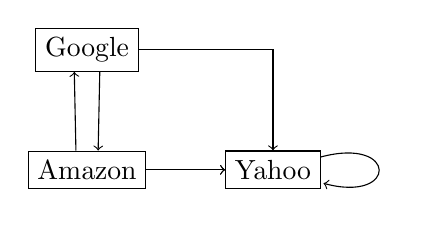
\begin{tikzpicture}
                        \node[rectangle, draw] (G) {Google};
                        \node[rectangle, draw, below= of G] (A) {Amazon};
                        \node[rectangle, draw, right= of A] (Y) {Yahoo};

                        \draw[->] (G) -| (Y);
                        \draw[->] (G.300) -- (A.60);
                        \draw[<-] (G.240) -- (A.120);
                        \draw[->] (A) -- (Y.180);
                        \draw[->] (A) -- (Y.180);
                        \draw[->, loop right] (Y) edge[loop right] (Y);
                    \end{tikzpicture}\\
                    PageRank is lost after each round and $\forall_i rank_i = 0$ & 
                    PageRank is accumulates on Yahoo and $\forall_i rank_i = 0$ behalf 
                    $rank_{yahoo} = 1$
                \end{tabular}

            \item \textsc{Improved PageRank}
                $$rank_i = 1-d + d \sum_{j \in B_i} \frac{1}{N_j} rank_j \quad \textrm{where }N_i \textrm{ is
                the outgoing link of i and} B_i \textrm{ the ingoing link of i}$$ 
        \end{itemize}

        \begin{description}
            \item[Init]: page $p <1/Nn, \{outgoingLink\}>$
            \item[Map]: page $p$ propagate $\frac{1}{N_p} * d * weigth_p$
            \item[Reduce]: page $p$ = $1-d + \sum_{incomingWeight}$
        \end{description}

\end{itemize}




\section{Hadoop}
\input{parts/05-hadoop}

\section{Batch processing}
\input{parts/06-batch}

\section{Stream processing}
\input{parts/07-stream}

\section{Data Center Galaxy}
\input{parts/08-galaxy}

\section{Web programming}
\input{parts/09-web}

\section{Behavioural tracking}
\input{parts/10-tracking}

\section{Distributed Systems Coordination}
\input{parts/11-distributed}

\section{Raft}
\input{parts/12-raft}


\section{Summary of Above the clouds: A berkeley view of cloud computing}
TODO

\section{Summary of Eventually Consistent}
\input{paper/eventually}

\section{Summary of Dynamo: Amazon’s Highly Available Key-value Store}
\input{paper/KVS}

\section{Summary of The Google File System (GFS)}
\input{paper/GFS}

\section{Summary of Pregel: A System for Large-Scale Graph Processing}
\input{paper/pregel}

\section{Summary of Resilient Distributed Datasets: A Fault-Tolerant Abstraction for In-Memory Cluster Computing}
\input{paper/resilient}

\section{Summary of Towards Predictable Datacenter Networks}

Since tenants pay based on the time they occupy their
VMs, and this time is influenced by the network, tenants
implicitly end up paying for the network traffic; yet, such
communication is supposedly free (hidden cost).

\subsection{Virtual Network Abstractions}

The “virtual” nature of the network implies that the provider
has a lot of freedom in terms of the topology of this
network, and can offer different options to tenants for different
costs. Beyond the overarching goal of maintaining the
simplicity of the interface between tenants and providers,
our topologies or virtual network abstractions are guided by
two design goals:

\begin{description}
\item[Tenant suitability] The abstractions should allow tenants
to reason in an intuitive way about the network performance
of their applications when running atop the virtual
network.
\item[Provider flexibility] Providers should be able to multiplex
many virtual networks on their physical network.
The greater the amount of sharing possible, the lesser
the tenant costs.
\end{description}

To this effect, we propose two novel abstractions for virtual
networks in the following sections.

\subsubsection{Virtual Cluster}

\includegraphics[width=0.8\linewidth]{img/virt_switch.png}

With a virtual cluster, a tenant request
<N, B> provides the following topology: each tenant
machine is connected to a virtual switch by a bidirectional
link of capacity B, resulting in a one-level tree topology. The
virtual switch has a bandwidth of $N \times B$. This ensures that
the virtual network has no oversubscription and the maximum
rate at which the tenant VMs can exchange data is
$N \times B$. However, this data rate is only feasible if the communication
matrix for the tenant application ensures that each VM sends and receives at rate B. Alternatively, if all N
tenant VMs were to send data to a single destination VM,
the data rate achieved will be limited to B.
Since a virtual cluster offers tenants a network with no
oversubscription, \textbf{it is suitable for data-intensive applications
like MapReduce and BLAST}. For precisely such applications,
Amazon’s Cluster Compute provides tenants with
compute instances connected through a dedicated 10 Gbps
network with no oversubscription. This may be regarded as
a specific realization of the virtual cluster abstraction with
<N , 10 Gbps>.

\subsubsection{Virtual Oversubscribed Cluster}

\includegraphics[width=0.8\linewidth]{img/virt_over_subscribed.png}

While a network with no oversubscription is imperative
for data-intensive applications, this does not hold for many
other applications [19,34]. Instead, a lot of cloud bound applications
are structured in the form of components with
more intra-component communication than inter-component
communication [16,25]. A “Virtual Oversubscribed Cluster”
is better suited for such cases; it capitalizes on application
structure to reduce the bandwidth needed from the underlying
physical infrastructure compared to virtual clusters,
thereby improving provider flexibility and reducing tenant
costs.

With a virtual oversubscribed cluster, a tenant request
<N , B, S, O>. Tenant
machines are arranged in groups of size S, resulting in $\frac{n}{s}$ groups. VMs in a group are connected by bidirectional links
of capacity $B$ to a (virtual) group switch. The group switches
are further connected using a link of capacity $B' = \frac{S \times B}{O}$ 
to a (virtual) root switch. The resulting topology has no oversubscription
for intra-group communication. However, intergroup
communication has an oversubscription factor $O$, i.e.,
\textbf{the aggregate bandwidth at the VMs is $O$ times greater than
the bandwidth at the root switch}. Hence, this abstraction
closely follows the structure of typical oversubscribed datacenter
networks. Note, however, that $O$ neither depends upon
nor requires physical topology oversubscription. Compared to virtual cluster, this abstraction does not offer
as dense a connectivity. However, the maximum data rate
with this topology is still $N \times B$.

The localized nature of the
tenant’s bandwidth demands resulting from this abstraction
allows the provider to fit more tenants on the physical network.
This, as our evaluation shows, has the potential to
significantly limit tenant costs. By incentivizing tenants to
expose the flexibility of their communication demands, the abstraction achieves better multiplexing which benefits both
tenants and providers. Amazon’s EC2 Spot Instances is
a good example of how tenants are willing to be flexible, especially
when it suits their application demands, if it means
lowered costs.

\includegraphics[width=0.7\linewidth]{img/net_comp.png}

\subsection{Oktopus}

With Oktopus,
tenants requesting VMs can opt for a (virtual) cluster or a
(virtual) oversubscribed cluster to connect their VMs.

 Two main components are used:

 \begin{description}
 \item[Management plane] A logically centralized network manager
(NM), upon receiving a tenant request, performs
admission control and maps the request to physical machines.
This process is the same as today’s setup except
that the NM needs to further account for network resources
and maintain bandwidth reservations across the
physical network.
\item[Data plane] Oktopus uses rate-limiting at endhost hypervisors
to enforce the bandwidth available at each VM.
This ensures that no explicit bandwidth reservations at
datacenter switches are required.
 \end{description}

 The network manager implements allocation algorithms
to allocate slots on physical machines to tenant requests in
an online fashion. For tenant requests involving a virtual
network, the NM needs to ensure that the corresponding
bandwidth demands can be met while maximizing the number
of concurrent tenants. To achieve this, the NM maintains
the following information :
\begin{itemize}
\item The datacenter network
topology
\item The residual bandwidth for each link in the
network
\item The empty slots on each physical machine
\item The allocation information for existing tenants,
including the physical machines they are allocated to, the
network routes between these machines and the bandwidth
reserved for the tenant at links along these routes
\end{itemize}

\subsection{End.}

See algorithm in the paper for allocation process, etc.





\section{Summary of Big Data: Principles and best practices}
TODO

\section{Summary of ZooKeeper: Wait-free coordination for Internet-scale systems}
\input{paper/Zookeeper}

\section{Summary : In Search of an Understandable Consensus Algorithm}
\input{paper/Consensus}

\section{Inginious questions}
\input{parts/Inginious}

\end{document}
